%%%%%%%%%%%%%%%%%%%%%%%%%%%%%%%%%%%%%%%%%
% License:
% CC BY-NC-SA 4.0 (http://creativecommons.org/licenses/by-nc-sa/4.0/)
%%%%%%%%%%%%%%%%%%%%%%%%%%%%%%%%%%%%%%%%%

%---------------------------------------------------
%	PACKAGES AND THEMES
%---------------------------------------------------

\documentclass[beamer]{beamer}

\mode<presentation> {

\usetheme{Madrid}

% Burnt orange
\definecolor{burntorange}{rgb}{0.8, 0.33, 0.0}
\colorlet{beamer@blendedblue}{burntorange}
% Pale yellow
\definecolor{paleyellow}{rgb}{1.0, 1.0, 0.953}
\setbeamercolor{background canvas}{bg=paleyellow}
% Secondary and tertiary palett
\setbeamercolor*{palette secondary}{use=structure,fg=white,bg=burntorange!80!black}
\setbeamercolor*{palette tertiary}{use=structure,fg=white,bg=burntorange!60!black}

% To remove the footer line in all slides uncomment this line
%\setbeamertemplate{footline}
% To replace the footer line in all slides with a simple slide count uncomment this line
%\setbeamertemplate{footline}[page number]

% To remove the navigation symbols from the bottom of all slides uncomment this line
%\setbeamertemplate{navigation symbols}{}
}


\usepackage{graphicx} % for figures
\usepackage{subcaption} % for subplots 
\usepackage[labelsep=space,tableposition=top]{caption}
\renewcommand{\figurename}{Fig.} 
\usepackage{cleveref}
\usepackage{booktabs} % Allows the use of \toprule, \midrule and \bottomrule in tables

%----------------------------------------------------------------------------------------
%	TITLE PAGE
%----------------------------------------------------------------------------------------
% The short title appears at the bottom of every slide, the full title is only on the title page
\title[CE394M: Geotechnical modeling]{CE394M: Advanced Analysis in Geotechnical Engineering} 

\author{Krishna Kumar} % name
\institute[UT Austin] % institution 
{
University of Texas at Austin \\
\medskip
\textit{
  \url{krishnak@utexas.edu}} % Your email address
}
\date{\today} % Date, can be changed to a custom date

\begin{document}

\begin{frame}
\titlepage % title page as the first slide
\end{frame}

\begin{frame}
 % Table of contents slide, comment this block out to remove it
 \frametitle{Overview}
 % Throughout your presentation, if you choose to use \section{} and \subsection{} 
 % commands, these %will automatically be printed on this slide as an overview 
 \tableofcontents
\end{frame}

%----------------------------------------------------------------------------------------
% slides
%----------------------------------------------------------------------------------------

%------------------------------------------------
\section{Geotechnical modeling}
%------------------------------------------------

\subsection{Complexity in Geotechnical modeling}
%------------------------------------------------
\begin{frame}
\frametitle{Geotechnical modeling of the complex world}
\begin{figure}
	\mode<handout>{
		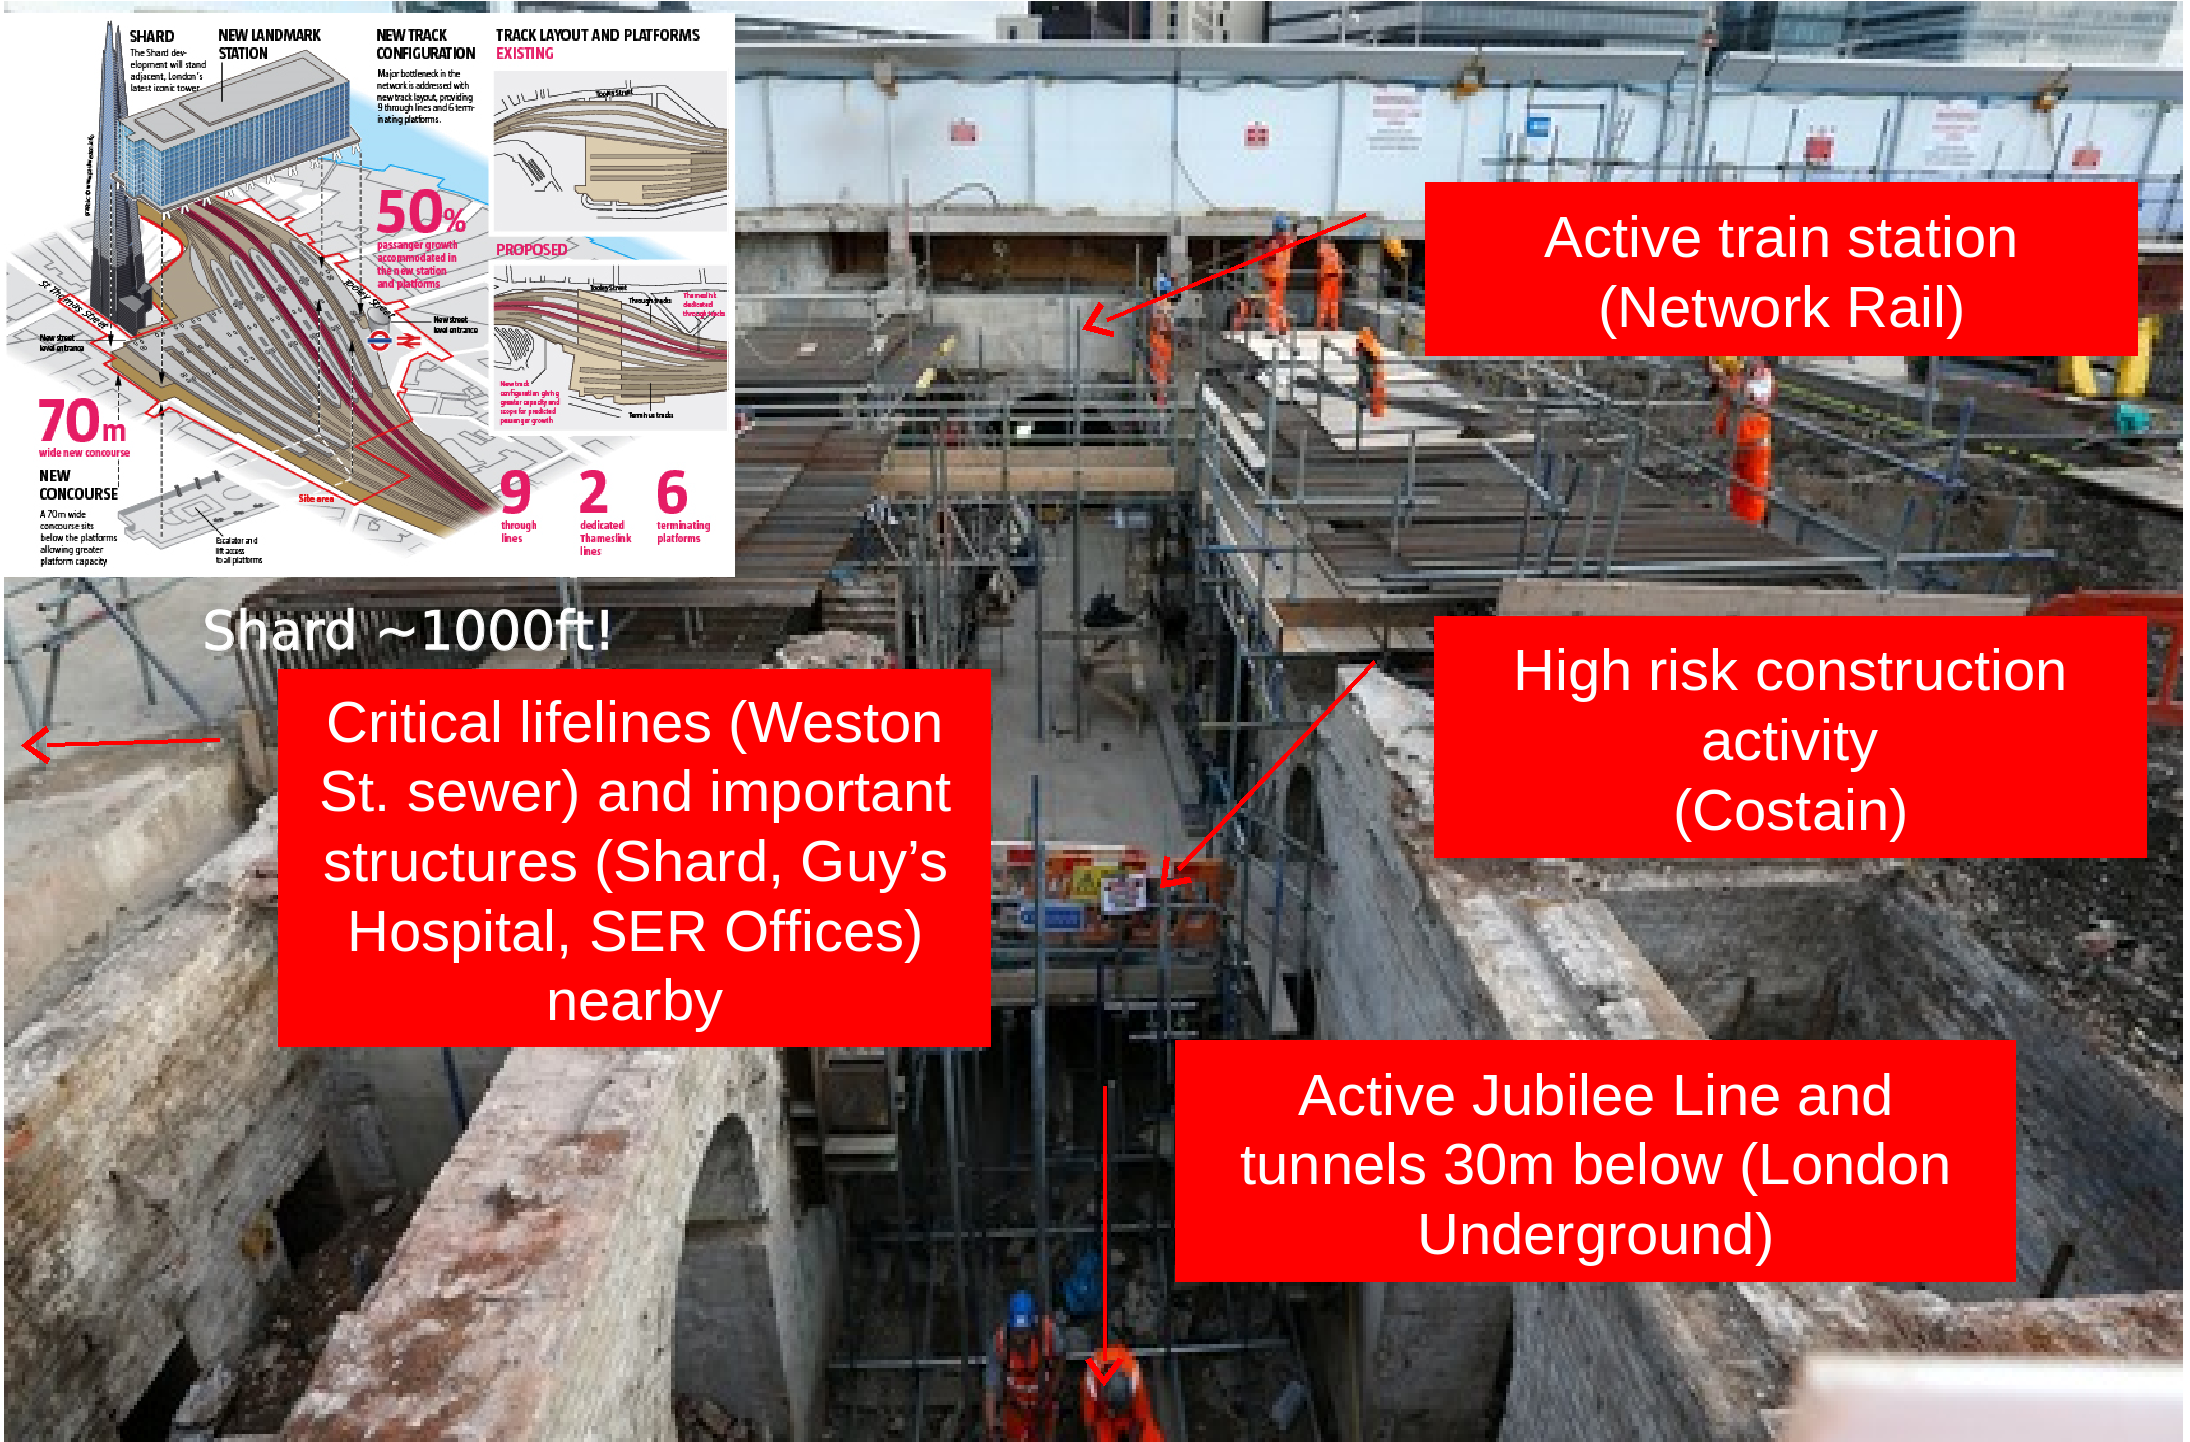
\includegraphics[width=0.85\textwidth]{figs/lbs.png}
	}
	\mode<beamer>{
		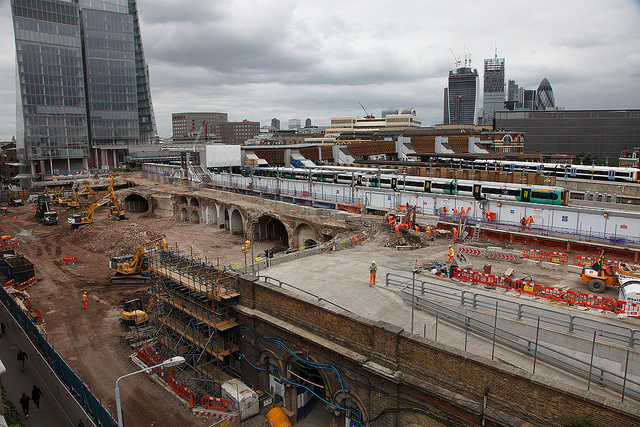
\includegraphics[width=0.85\textwidth]{figs/lbs-overview.jpg}
	}
	\caption{London Bridge Station, London, UK}
\end{figure}
\end{frame}

%------------------------------------------------
\begin{frame}
\frametitle{Geotechnical modeling of the complex world}
\begin{figure}
	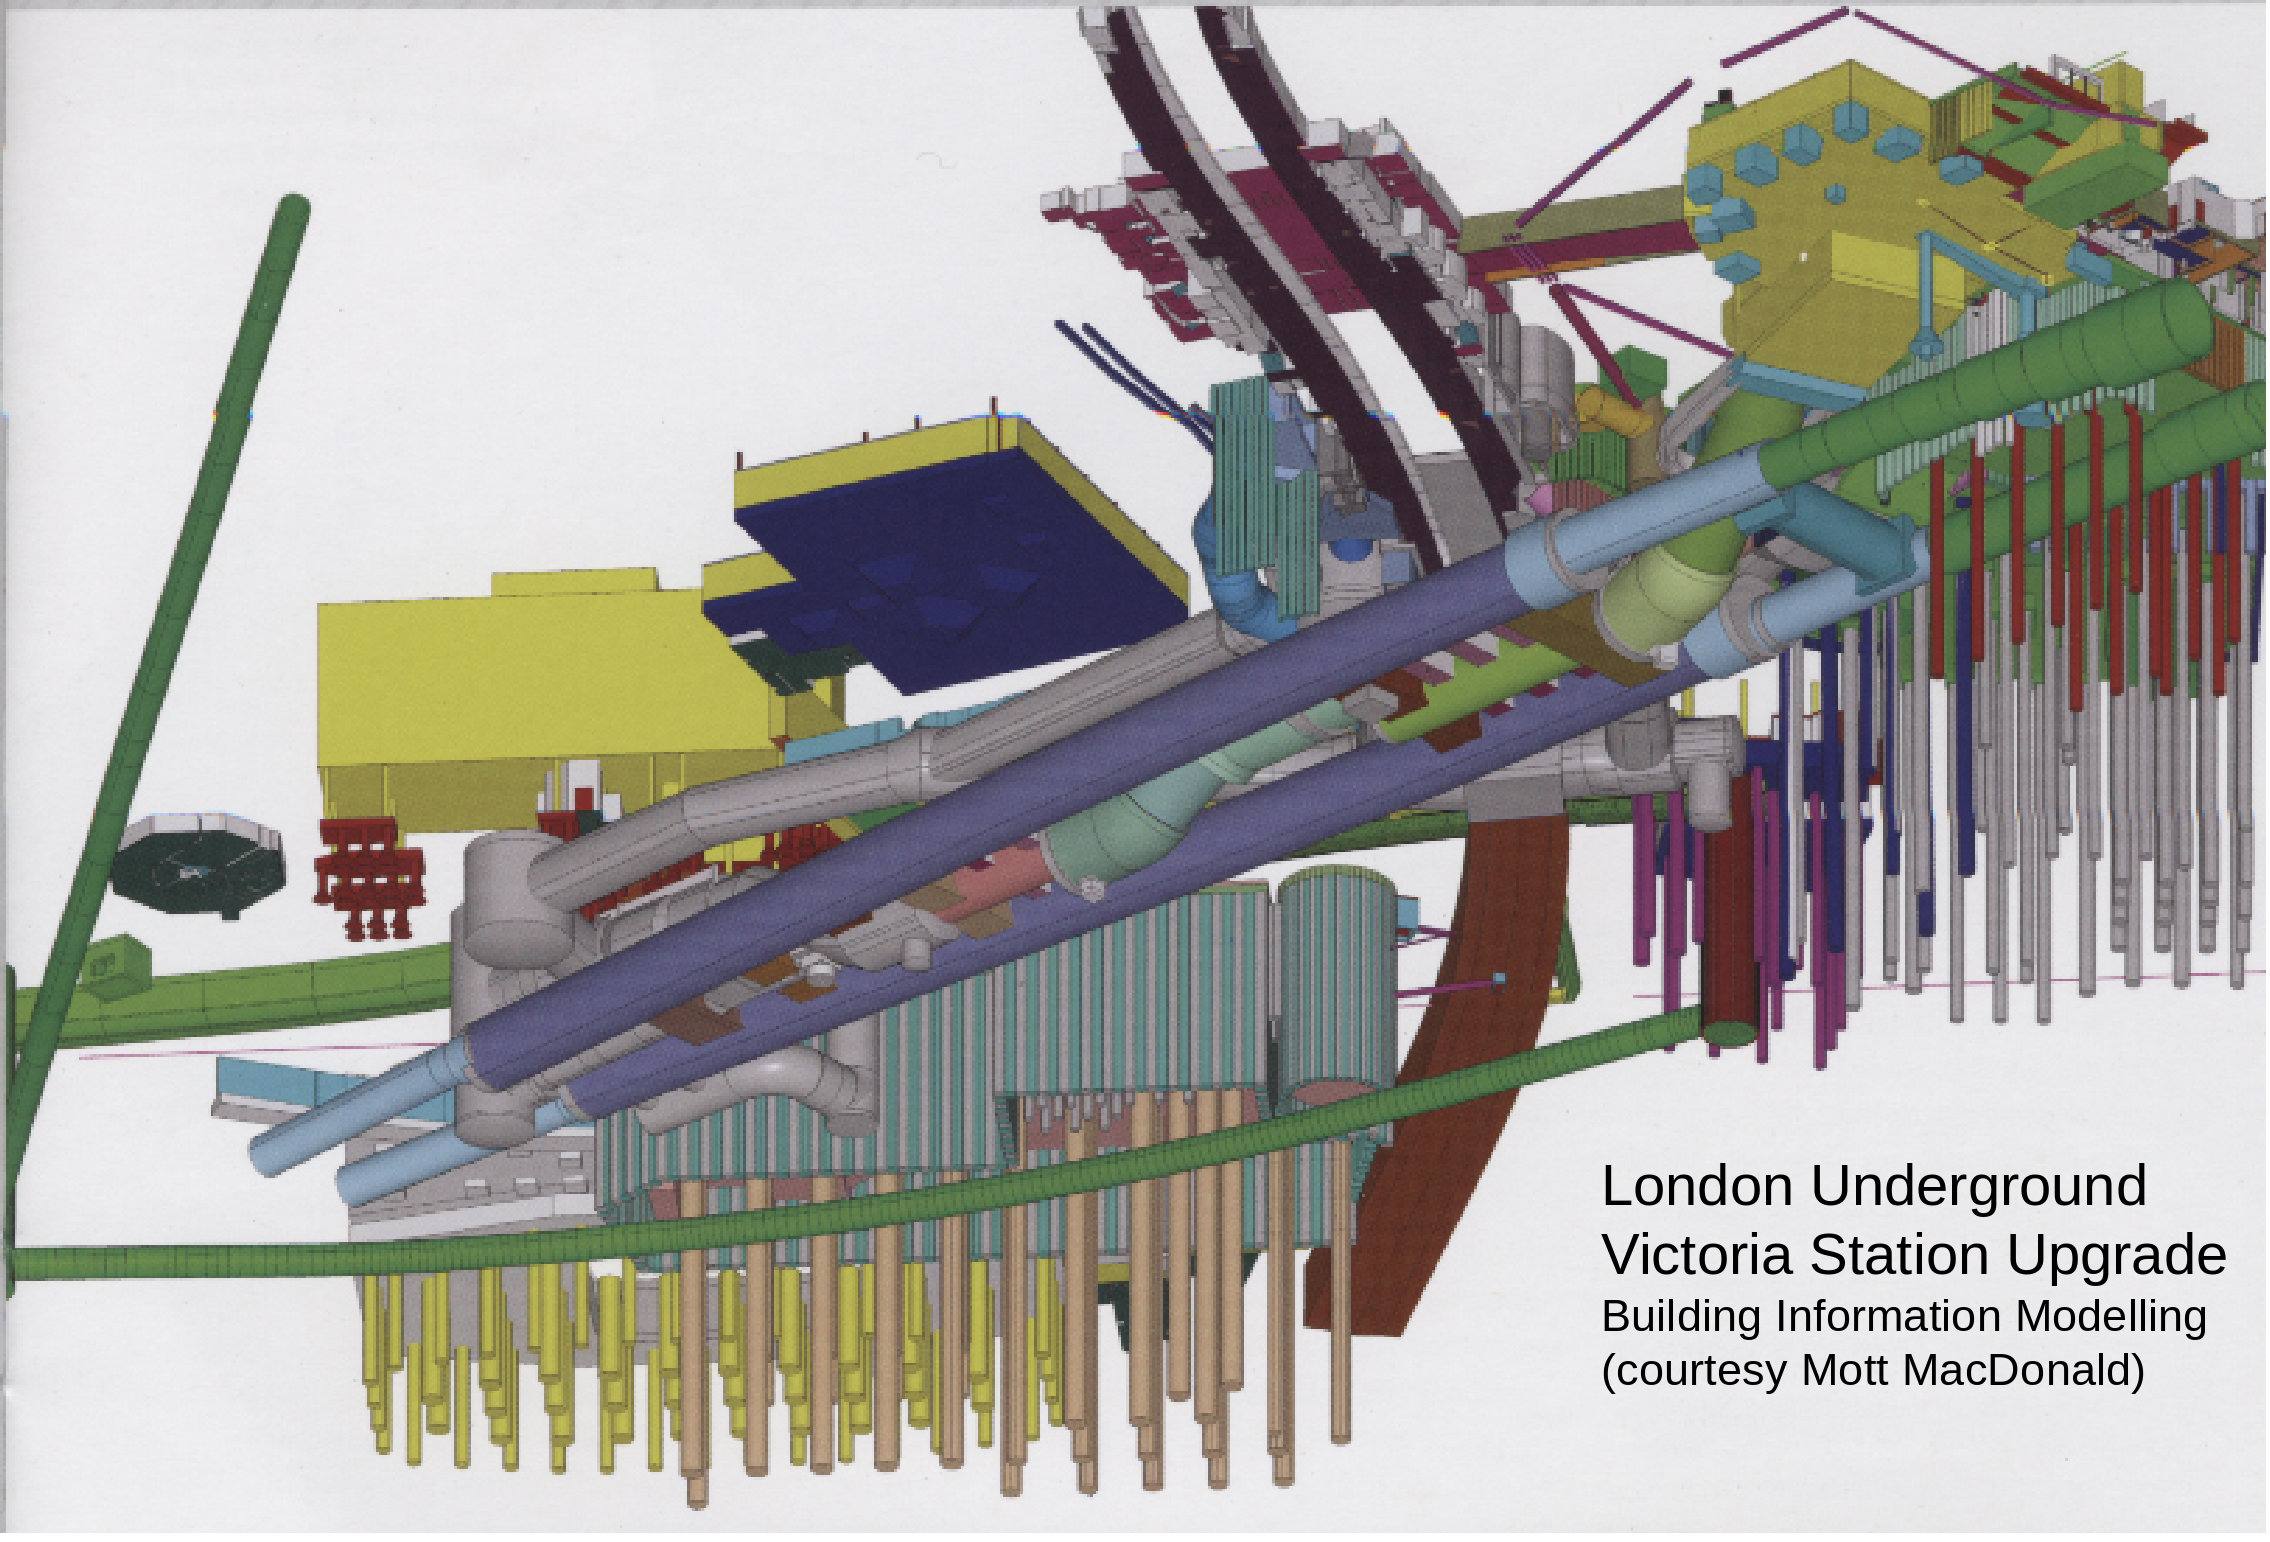
\includegraphics[width=0.85\textwidth]{figs/victoria-station.png}
	\caption{London Victoria station upgrade, London, UK}
\end{figure}
\end{frame}

%------------------------------------------------
\begin{frame}
\frametitle{Geotechnical modeling}
\begin{figure}
  \mode<handout>{
	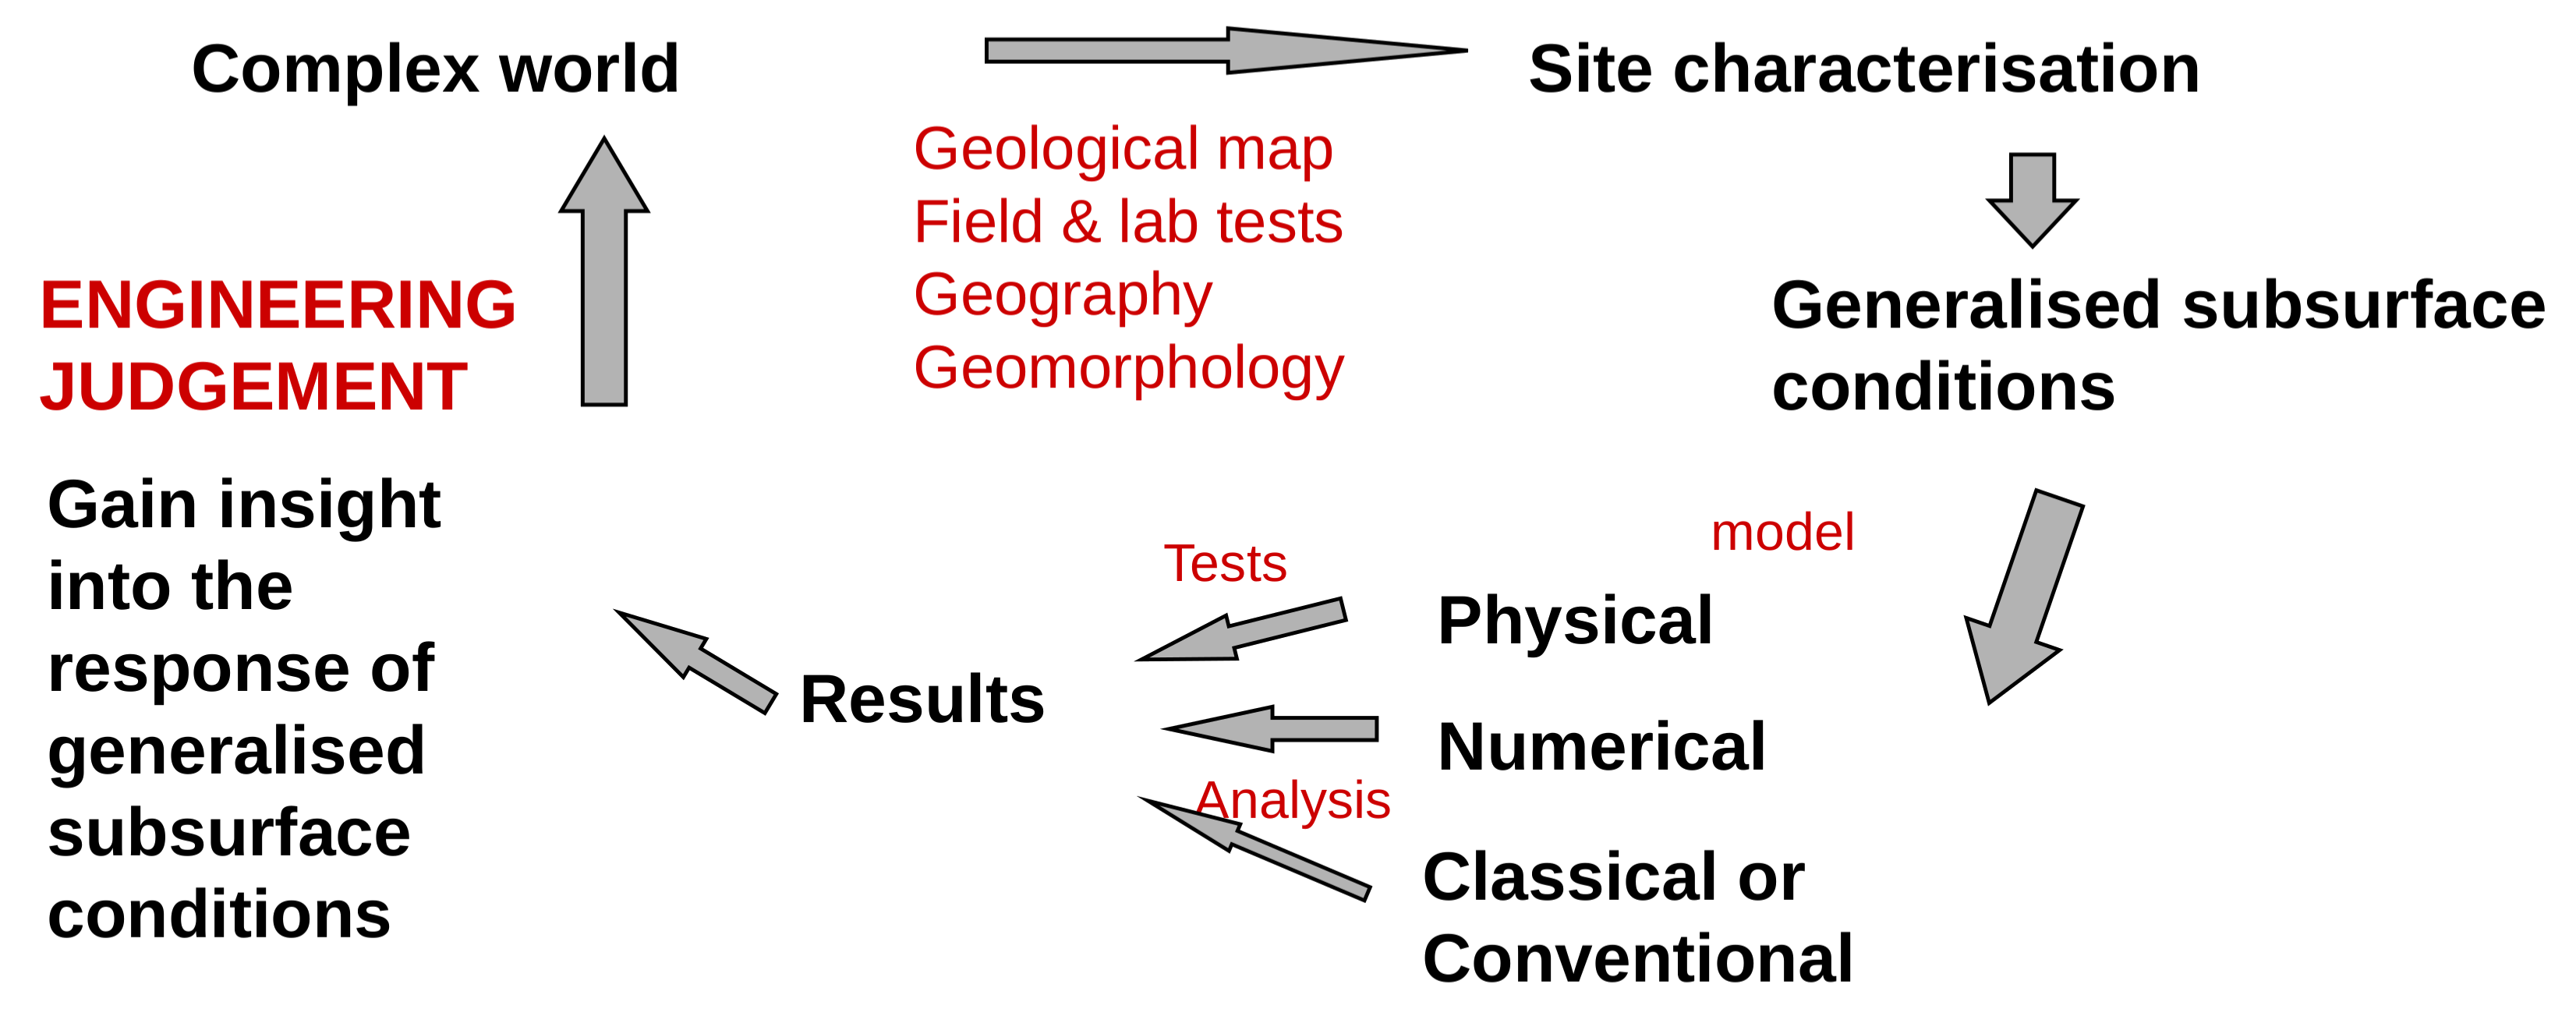
\includegraphics[width=0.85\textwidth]{figs/geotechnical-modeling-final.png}
  }
  \mode<beamer>{
	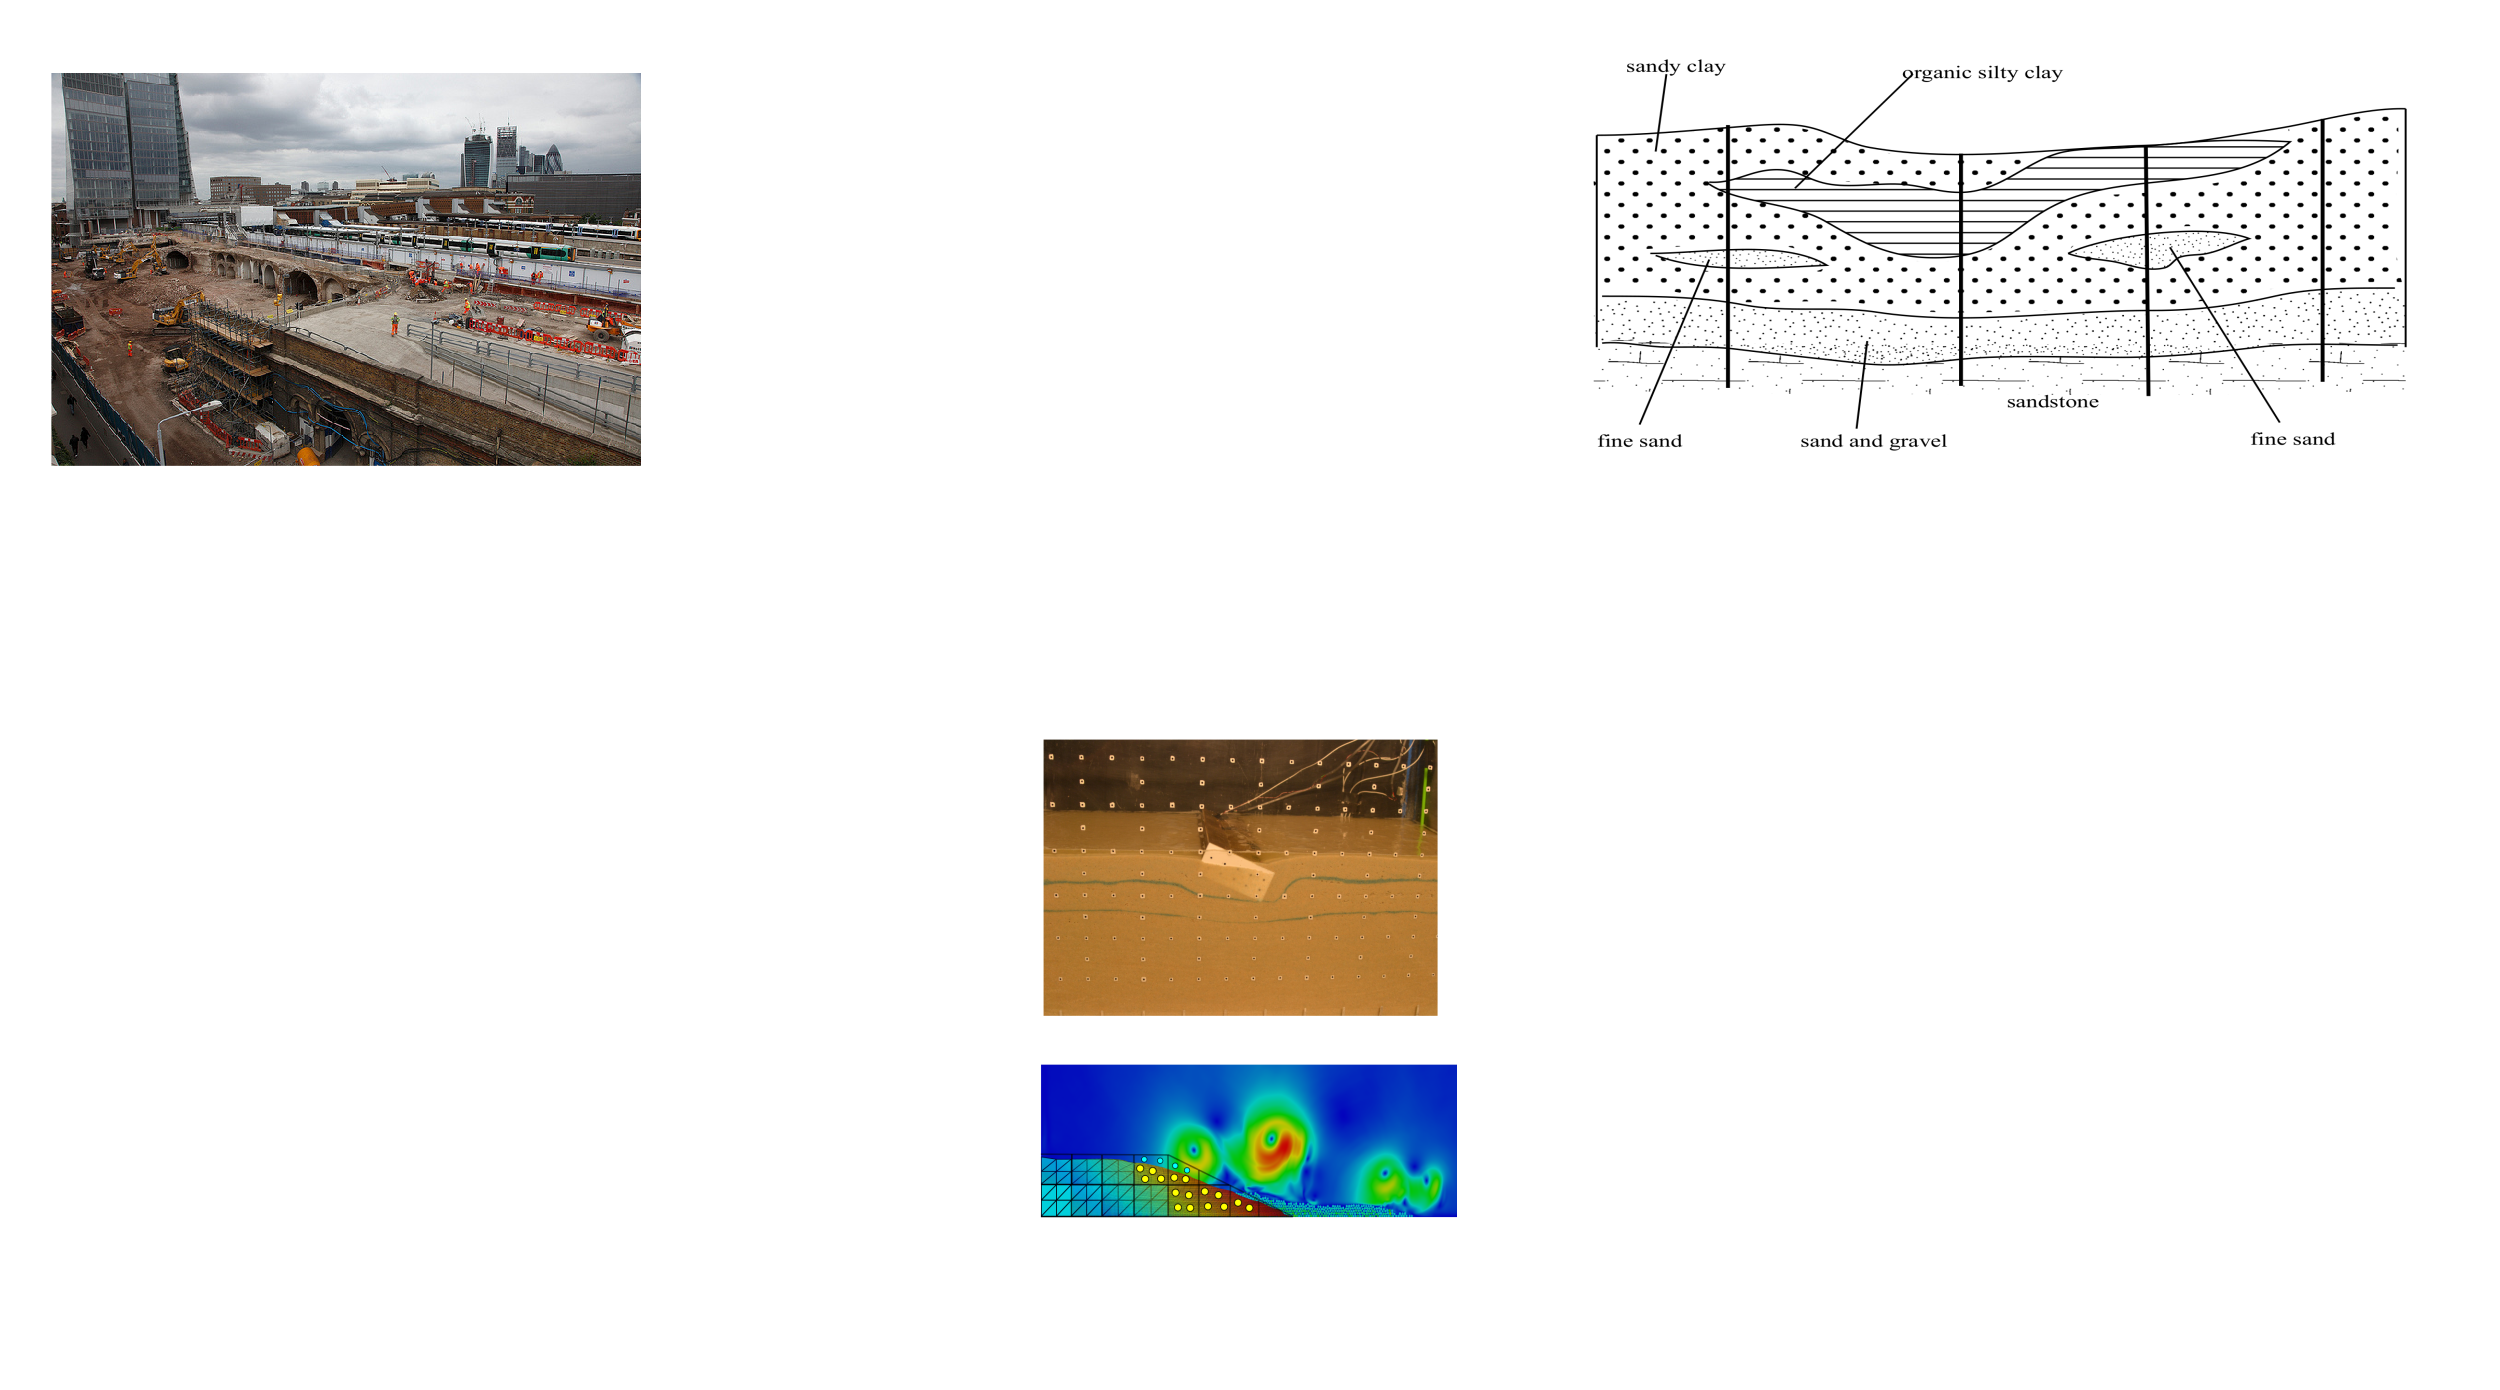
\includegraphics[width=0.95\textwidth]{figs/geotechnical-modeling.png}
  }
\end{figure}
\end{frame}

%------------------------------------------------
\begin{frame}
\frametitle{Soil behavior}
\begin{itemize}
	\item nonhomogeneous,
	\item anisotropic, 
	\item non-linear, 
	\item initial stress conditions, 
	\item stress history
	\item Geometry - very complex
\end{itemize}
\textbf{Soil Mechanics in practice - largely empirical}
\end{frame}

%------------------------------------------------
\begin{frame}
\frametitle{Geotechnical modeling}
\begin{itemize}
	\item Self weight effect of soils (This is why soil moves)
	\item Construction sequence (Complex geometry)
	\item Water movement (undrained, consolidation, drained)
	\item Insitu stresses (stiffness/strength depends on current stresses and stress history)
	\item Predict the ability of a design to withstand extreme loading conditions (you only have one chance)
\end{itemize}
\begin{figure}
	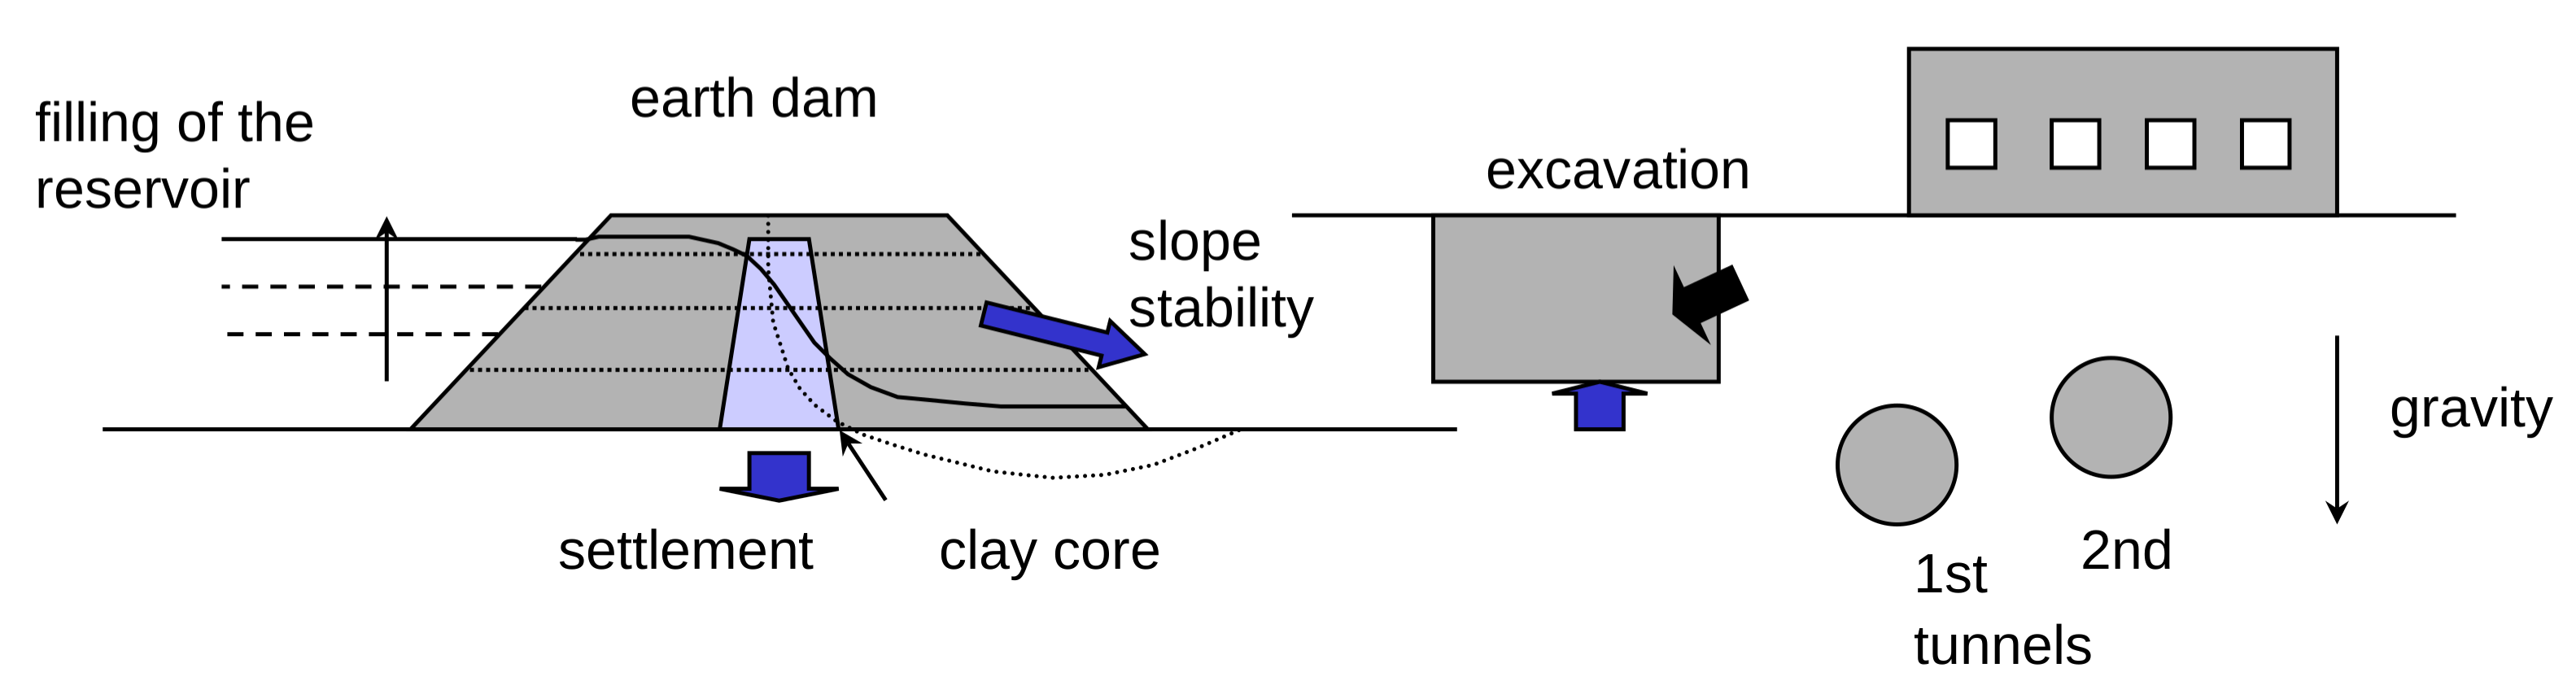
\includegraphics[width=0.95\textwidth]{figs/geotechnical-modeling-examples.png}
\end{figure}
\end{frame}

\end{document} 
